\documentclass[a4paper]{ctexart}
\usepackage{amsmath}
\usepackage{graphicx}
\usepackage{hyperref}
\usepackage{float}
\usepackage{geometry}
\title{测量金属的杨氏模量}
\author{陈启钰\,\,2300011447}
\date{\today}
\begin{document}
	\maketitle
	\tableofcontents
	\section{测量数据的整理}
	\subsection{测量金属丝的直径}
	\noindent 螺旋测微仪的零差为
	\begin{align}
		d_0=0.003\mathrm{mm}
	\end{align}
	\begin{table}[H]
		\begin{center}
			\caption{金属丝直径的测量}
			\begin{tabular}{c|cccccccccc}
				i&1&2&3&4&5&6&7&8&9&10\\
				\hline
				$d_i/\mathrm{mm}$&0.327&0.327&0.325&0.324&0.325&0.327&0.323&0.325&0.325&0.326
			\end{tabular}
		\end{center}
	\end{table}
	平均值
	\begin{align}
		\overline{d}=\frac{1}{10}\sum_{i=1}^{10}(d_i-d_0)=0.322\mathrm{mm}
	\end{align}
	不确定度的计算
	\begin{align}
		\sigma_a(\overline{d})&=\sqrt{\frac{1}{10\times9}\sum_{i=1}^{10}(d_i-d_0-\overline{d})^2}=0.0005\mathrm{mm}\\
		\sigma_b(\overline{d})&=\frac{0.004\mathrm{mm}}{\sqrt{3}}\\
		\sigma(\overline{d})&=0.003\mathrm{mm}
	\end{align}
	最后可得
	\begin{align}
		d=(0.322\pm 0.003)\mathrm{mm}
	\end{align}
	\subsection{金属丝长度的测量}
	单次测量结果为\footnote{此处不确定度为估计值,非计算值}
	\begin{align}
		\sigma_b(\overline{L})=\frac{0.15\mathrm{mm}}{\sqrt{3}}
	\end{align}
	\begin{align}
		L=(82.71\pm 0.09)\mathrm{cm}
	\end{align}
	\subsection{质量以及金属丝伸长量的测量}
	\begin{table}[H]
		\begin{center}
			\caption{砝码质量以及金属丝伸长量的测量}
			\begin{tabular}{c|cccccccccc}
				个数$i$&0&1&2&3&4&5&6&7&8&9\\\hline
				单个质量$m_i/\mathrm{g}$&/&199.85&199.97&200.11&199.90&199.88&200.28&199.83&200.00&199.72\\\hline
				总质量$m/\mathrm{g}$&0.00&199.85&399.82&599.93&799.83&999.71&1199.99&1399.82&1599.82&1799.54\\\hline
				$x_{up}/\mathrm{mm}$&4.03&3.90&3.76&3.63&3.51&3.40&3.28&3.15&3.04&2.92\\\hline
				$x_{down}/\mathrm{mm}$&4.04&3.90&3.80&3.67&3.53&3.44&3.29&3.17&3.04&2.93\\\hline
				$x_i/\mathrm{mm}$&4.035&3.900&3.780&3.650&3.520&3.420&3.285&3.160&3.040&2.925
			\end{tabular}
		\end{center}
	\end{table}
	值得注意的是,表中$x_i$的计算多保留了一位有效数字。
	\subsubsection{砝码质量的计算}
	\begin{align}
		\overline{m}&=\frac{1}{10}\sum_{i=0}^{9}m_i=199.95\mathrm{g}\\
		\sigma_a(\overline{m})&=\sqrt{\frac{1}{10\times9}\sum_{i=0}^{9}(m_i-\overline{m})^2}=0.056\mathrm{g}\\
		\sigma_b(\overline{m})&=\frac{0.02\mathrm{g}}{\sqrt{3}}\\
		\sigma(\overline{m})&=0.06\mathrm{g}
	\end{align}
	所以有
	\begin{align}
		m=(199.95\pm 0.06)\mathrm{g}
	\end{align}
	\subsubsection{逐差法计算金属丝伸长量}
	将所测得的数据两两配对,进行逐差法计算,$\Delta x_i=x_{i-1}-x_{i+4}(i=1,2,3,4,5)$
	\begin{table}[H]
		\begin{center}
			\caption{逐差法计算金属丝伸长量记录表}
			\begin{tabular}{c|ccccc}
				i&1&2&3&4&5\\\hline
				$\Delta x_i/\mathrm{mm}$&0.615&0.615&0.620&0.610&0.595
			\end{tabular}
		\end{center}
	\end{table}
	\begin{align}
		\overline{\Delta x}&=\frac{1}{5}\sum_{i=1}^{5}\Delta x_i=0.611\mathrm{mm}\\
		\sigma_a(\overline{\Delta x})&=\sqrt{\frac{1}{5\times4}\sum_{i=1}^{5}(\Delta x_i-\overline{\Delta x})^2}=0.0043\mathrm{mm}\\
		\sigma_b(\overline{\Delta x})&=\frac{0.05\mathrm{mm}}{\sqrt{3}}\\
		\sigma(\overline{\Delta x})&=0.03\mathrm{mm}
	\end{align}
	可得
	\begin{align}
		\Delta x=(0.61\pm 0.03)\mathrm{mm}
	\end{align}
	从而
	\begin{align}
		\delta L=\frac{1}{5}\Delta x=(0.122\pm 0.006)\mathrm{mm}
	\end{align}
	\section{逐差法计算杨氏模量}
	由杨氏模量的计算公式
	\begin{align}
		E=\frac{4mgL}{\pi d^2\delta L}
	\end{align}
	\begin{align}
		\overline{E}=\frac{4\overline{m}g\overline{L}}{\pi \overline{d}^2\overline{\delta L}}=1.63\times10^{11}\mathrm{Pa}
	\end{align}
	相对不确定度满足
	\begin{align}
		\frac{\sigma(\overline{E})}{\overline{E}}=\sqrt{\left(\frac{\sigma(\overline{m})}{\overline{m}}\right)^2+\left(\frac{\sigma(\overline{L})}{\overline{L}}\right)^2+\left(\frac{\sigma(\overline{\delta L})}{\overline{\delta L}}\right)^2+\left(\frac{2\sigma(\overline{d})}{\overline{d}}\right)}=0.053
	\end{align}
	\begin{align}
		\sigma(\overline{E})=0.09\times10^{11}\mathrm{Pa}
	\end{align}
	所以
	\begin{align}
		E=(1.63\pm 0.09)\times10^{11}\mathrm{Pa}
	\end{align}
	\section{用最小二乘法计算杨氏模量}
	\noindent 我们可以根据
	\begin{align}
		x_i=\frac{4mgL}{\pi d^2E}i+x_0\equiv ki+x_0
	\end{align}
	用最小二乘法线性拟合得到
	\begin{align}
		k=0.1231\mathrm{mm},r=0.9998
	\end{align}
	计算$k$的不确定度,由于$i$无误差,所以
	\begin{align}
		\sigma_a(k)=k\sqrt{\frac{1/r^2-1}{n-2}}=0.0009\mathrm{mm}
	\end{align}
	\begin{align}
		\sigma_b(k)=\sqrt{\sum_{i=0}^{9}\left(\frac{\partial k}{\partial x_i}\sigma(x_i)\right)^2}
	\end{align}
	对于任意的$i$和$j$,有
	\begin{align}
		\sigma(x_i)=\sigma(x_j)=\sigma=\frac{0.05\mathrm{mm}}{\sqrt{3}}
	\end{align}
	所以有
	\begin{align}
		\sigma_b(k)=\sqrt{\sigma^2\sum_{i=0}^{9}\left(\frac{x_i-\overline{x}}{\sum_{i=0}^{9}(x_i-\overline{x})^2}\right)^2}=\frac{\sigma}{\sqrt{\sum_{i=0}^{9}(x_i-\overline{x})^2}}=0.0032\mathrm{mm}
	\end{align}
	\begin{align}
		\sigma(k)=0.0033\mathrm{mm}
	\end{align}
	\begin{align}
		k=(0.1231\pm 0.0033)\mathrm{mm}
	\end{align}
	再计算杨氏模量
	\begin{align}
		\overline{E}=\frac{4\overline{m}g\overline{L}}{\pi \overline{d}^2\overline{k}}=1.62\times10^{11}\mathrm{Pa}
	\end{align}
	相对不确定度
	\begin{align}
		\frac{\sigma(\overline{E})}{\overline{E}}=\sqrt{\left(\frac{\sigma(\overline{m})}{\overline{m}}\right)^2+\left(\frac{\sigma(\overline{L})}{\overline{L}}\right)^2+\left(\frac{\sigma(\overline{k})}{\overline{k}}\right)^2+\left(\frac{2\sigma(\overline{d})}{\overline{d}}\right)}=0.032
	\end{align}
	\begin{align}
		\sigma(\overline{E})=0.06\times10^{11}\mathrm{Pa}
	\end{align}
	所以
	\begin{align}
		E=(1.62\pm0.06)\times10^{11}\mathrm{Pa}
	\end{align}
	当然,我们也可以根据图像直观观察线性关系\footnote{注意图中直线斜率为负!实际上在计算中我们已经取了绝对值。}
	\begin{figure}[H]
		\centering
		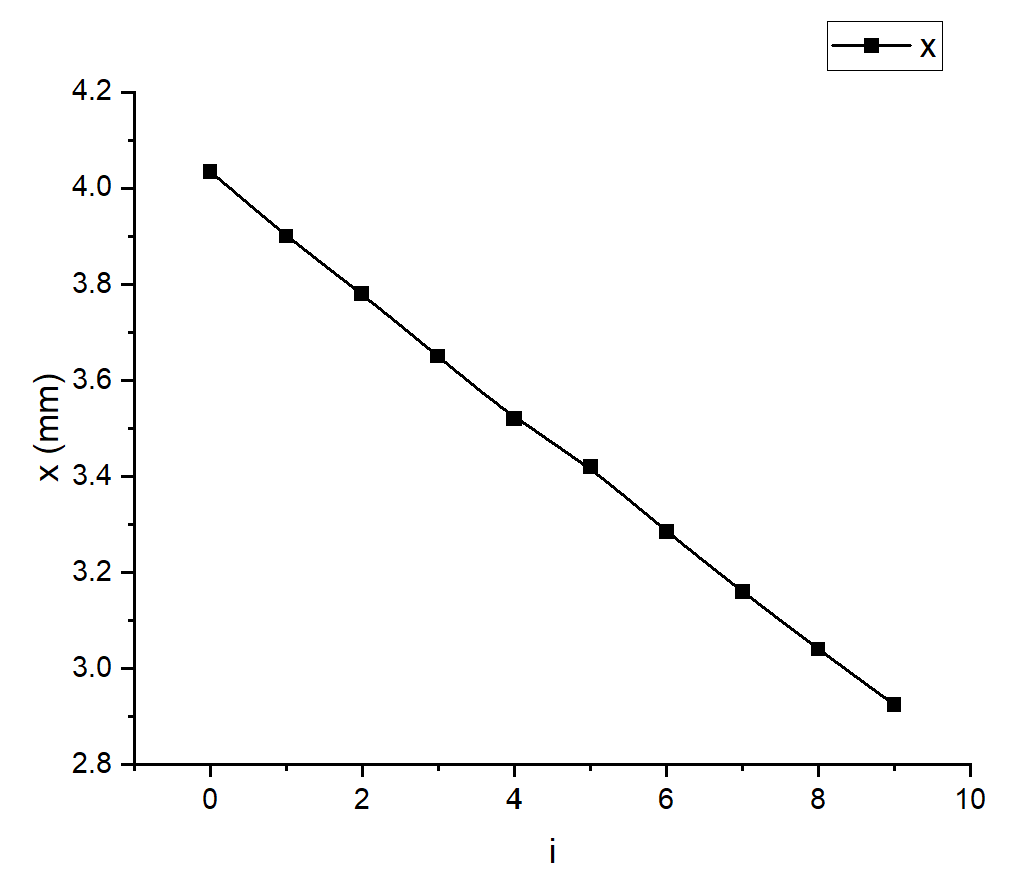
\includegraphics[width=8cm]{1.png}
		\caption{$x-i$图}
	\end{figure}
	\section{误差分析}
	我们来观察各个物理量的相对不确定度\\
	长度
	\begin{align}
		\frac{\sigma(L)}{L}=0.001
	\end{align}
	直径
	\begin{align}
		\frac{\sigma(d)}{d}=0.0093
	\end{align}
	质量
	\begin{align}
		\frac{\sigma(m)}{m}=0.0003
	\end{align}
	伸长量
	\begin{align}
		\frac{\sigma(\delta L)}{\delta L}=0.049
	\end{align}
	当然还有$k$
	\begin{align}
		\frac{\sigma(k)}{k}=0.027
	\end{align}
	显然地有大小关系
	\begin{align}
		\frac{\sigma(\delta L)}{\delta L}\sim\frac{\sigma(k)}{k}\gg\frac{\sigma(d)}{d}\gg\frac{\sigma(L)}{L}\sim\frac{\sigma(m)}{m}
	\end{align}
	所以,误差的最大来源是伸长量的测量。\\
	为什么伸长量的测量会带来如此大的相对误差?首先有钢丝本身的问题,因为钢丝的伸长是需要一定时间的,而且周围环境因素的影响会导致钢丝的伸长没有理想中那么线性,导致A类不确定变大。仪器方面也会有影响,因为我们计算B类不确定度时将仪器允差估计为$0.05\mathrm{mm}$,远大于A类不确定度,也就是说仪器允差是伸长量不确定度的主要来源。因此,如果我们想要有更精确的测量结果,应该更换更精密的仪器。
	\section{原始数据}
	\begin{figure}[H]
		\centering
		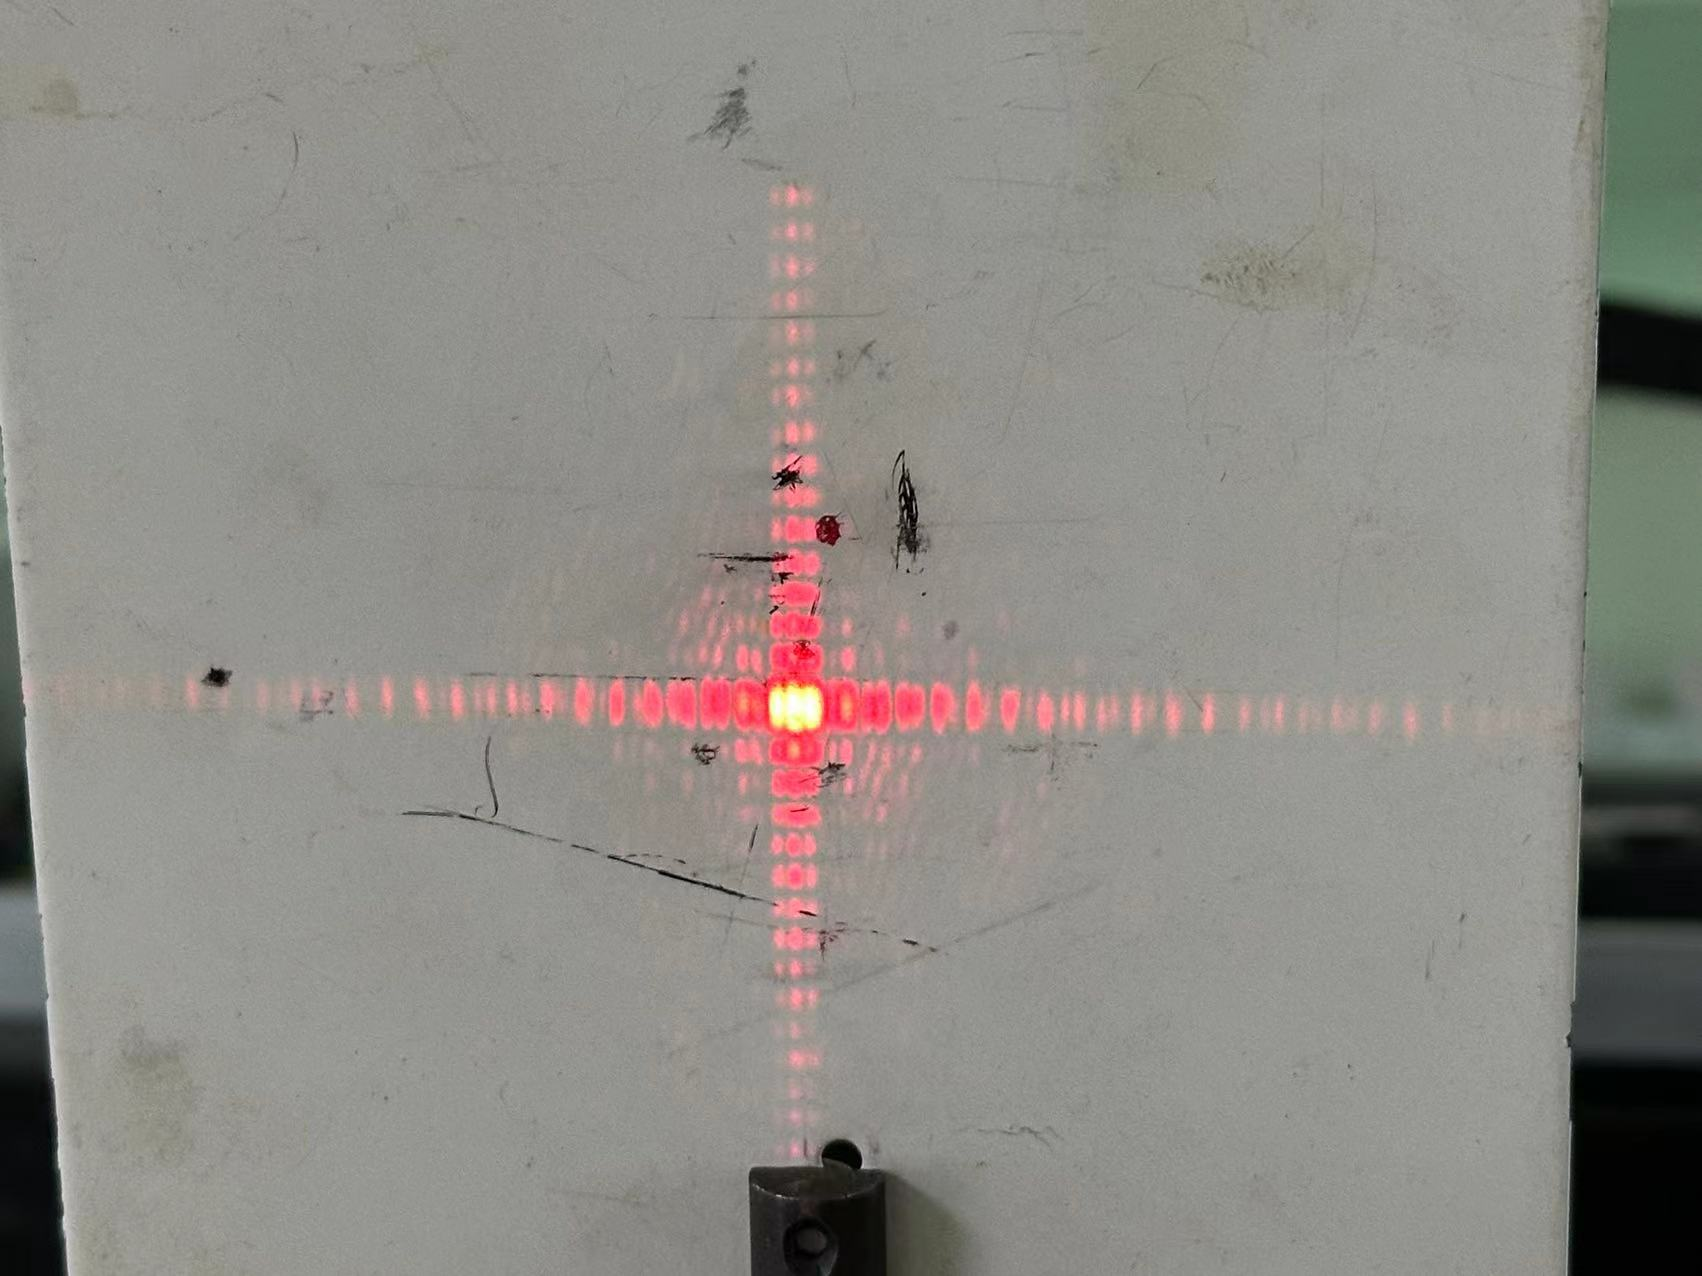
\includegraphics[width=13cm]{2.jpg}
	\end{figure}
\end{document}